
\section*{Notas y Pruebas} % Espacio para hablar del proyecto de maestría de Marianne, 

%% Escribir lo que sigue de alguna otra manera. 

\textit{Notas de Ausencia} \citep{notasdeausencia} es un ensayo generativo en la web. Utiliza el texto dato que por medio de la computadora como agente resignificante, deconstruye estructuras discursivas para resemantizar la narrativa sobre las desapariciones de mujeres en México y América Latina.

El tiempo y espacio virtual conforman una partitura para la memoria y la denuncia. La narrativa, semi autónoma, argumenta a partir de textos tomados de tweets, poemarios, libros y artículos feministas que explican desde la teoría las desapariciones forzadas, el feminicidio y la violencia de género. Lo cuales están presente como texto, imagen y sonido en un espacio tridemencional diseñado para funcionar a manera de memorial.

La narrativa de la pieza está articulada mediante la intervención de dos bots. El primero comparte tuits que localiza con hashtag como: \#MéxicoFeminicida, \#MadresEnBúsqueda, \#ViolenciadeGenero, \#NiUnaMenos, entre otros.\footnote{\url{https://twitter.com/notasausencia} (Consultado el \today)} Así como con un bot de generación de texto automático que remixea los textos selecionados por medio de cadenas de Markov.

\begin{figure}[H]
  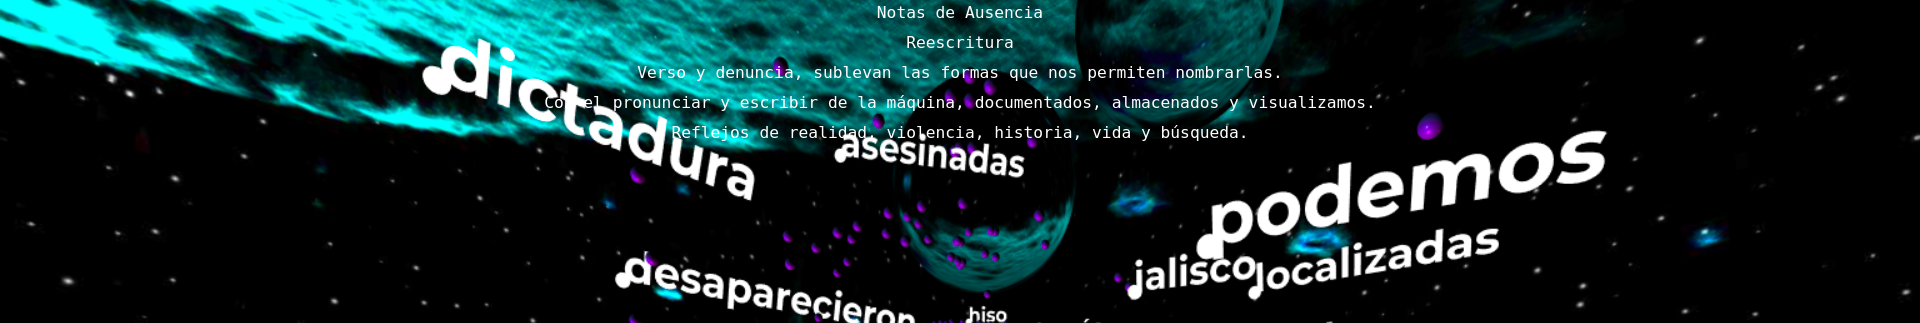
\includegraphics[width=\textwidth]{img/notas.png}
  \caption{Notas de Ausencia de Marianne Teixido}
\end{figure}

Esta pieza se realizó en el contexto de la exhibición en línea Creaciones con algoritmos: visualización y sonificación de datos del Centro de Cultura Digital en abril de 2020. Su salida oficial se realizó en video sin embargo, el planeamiento original contempló la creación de un espacio virtual en la web que pudiera visualizar en tiempo real la información viva proveniente de los tweets. 
En respuesta a la necesidad de ubicar la pieza en una espacio tridimencional en la web, en colaboración con \textit{PiranhaLab} se planeó el uso de Three.js como solución para conectar dicho espacio y con la información proporcionada por los bots. 

A raíz de dicho proceso artístico generamos las condiciones técnicas referentes a la relativa autonomía del servidor requerido para mantener la pieza en línea, la cual permanece activa.

Por otro lado \textit{Pruebas Proféticas} fue el evento piloto que implementó por primera vez dos tipos de tecnologías específicas: exploración multijugador y \textit{streaming} personalizado, montados en un escenario tridimensional previamente explorado en Notas de Ausencia. 

\begin{figure}[H]
  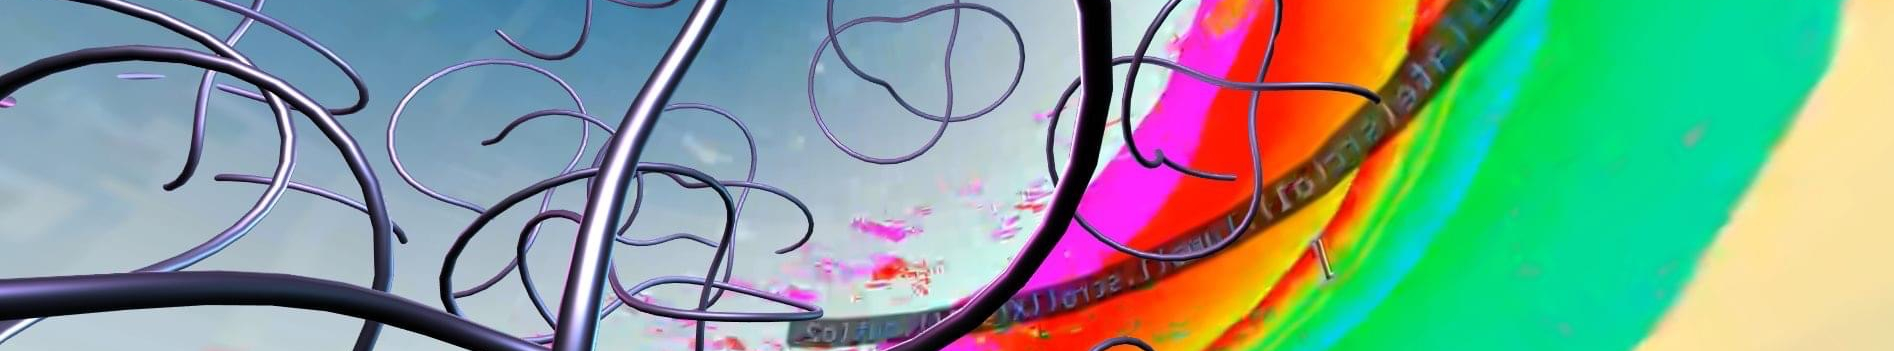
\includegraphics[width=\textwidth]{img/pruebasprofeticas.jpg}
  \caption{Pruebas proféticas. Visuales: Flor de Fuego}
\end{figure}

%La transmisión de audio y video fue un aspecto que el planteamiento de \textit{PiranhaLab} buscó solucionar. Es posible utilizar servicios gratuitos o de paga para la transmisión de datos audiovisuales, sin embargo, en menor o mayor medida, el flujo audiovisual generado es analizado y en caso de que se detecte algún extacto de audio proveniente con derechos de autor, el stream es silenciado. Este artículo no busca centrarse en discusiones sobre derechos de autor sino en la usabilidad de un streaming audiovisual. 


 \color{Fuchsia}

La experiencia con \textit{Pruebas Proféticas} abrió camino para el diseño de la edición 2020 de EDGES. Durante el proceso el proyecto nos permitió reflexionar en torno a funcionalidad y experimentación como dos posibilidades de un continuo para la escritura de software en un marco artístico y performático. EDGES como plataforma explicita el papel experimental de los actos, la plataforma tecnológica también podría ser experimental e incluso podría desdibujarse en pos de la integración performance-espacio bajo la misma premisa de la experimentación.

\color{black}

El concepto curatorial de \textit{EDGES} estuvo definido por Marianne Teixido y guardó una estrecha relación con los planteamientos de \textit{Notas de Ausencia}, considera las posibilidades de creación planteandonos desde el feminismo intereseccional, perspectiva desde la cual se problematiza el uso de la tecnología teniendo en consideración las condiciones de raza, género y clase, a partir de la cuales se establece una crítica las herramientas hegemónicas ya dadas para apuntar a la creación de estas otras herramientas, construídas desde dinámicas de organización colectiva y conocimientos situados. \textit{EDGES 2020} como propuesta curatorial contempla la participación en su mayoría de mujeres y persona no binaries. Las obras dialogan con las hibridaciones e-corporales en espacios virtuales ficcionados desde las subjetividades feministas y transfeministas que toman internet como territorio y espacio de intercambio cultural.

\iffalse
- Uso de espacios tridimensionales 
- Bots y literatura 
- Datos que transforman el espacio   
- Ensayos digitales en la web
- cyberfeminisimo
- audio virtualmente posicionado 
- streaming de audio y video sin plataformas privativas - decisiones de optimización
- Según yo aquí usamos icecast y liquid soap 
- Inicios de multiplayer
\fi
